
%(BEGIN_QUESTION)
% Copyright 2006, Tony R. Kuphaldt, released under the Creative Commons Attribution License (v 1.0)
% This means you may do almost anything with this work of mine, so long as you give me proper credit

En type væskenivåbryter kalt \textit{tilt switch} brukes ofte for å detektere kloakknivå i ``lift stations'', der avløp samlet fra boliger via gravitasjon pumpes videre til renseanlegg (ofte flere kilometer unna):

$$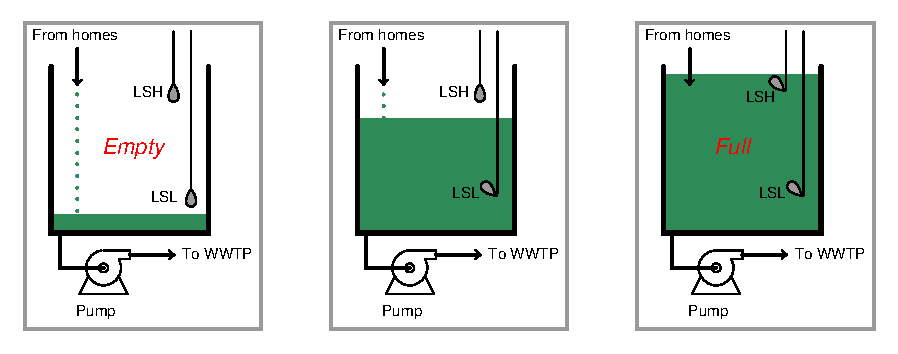
\includegraphics[width=15.5cm]{i00303x01.eps}$$

Tilt-brytere bruker ofte et lite glassrør med flytende kvikksølv som tilt-sensor.  Forklar hvordan et glassrør delvis fylt med kvikksølv fungerer som elektrisk tilt-bryter, og gjør et tankeeksperiment der du beskriver funksjonen gjennom en komplett start-stopp-syklus av pumpemotoren:

$$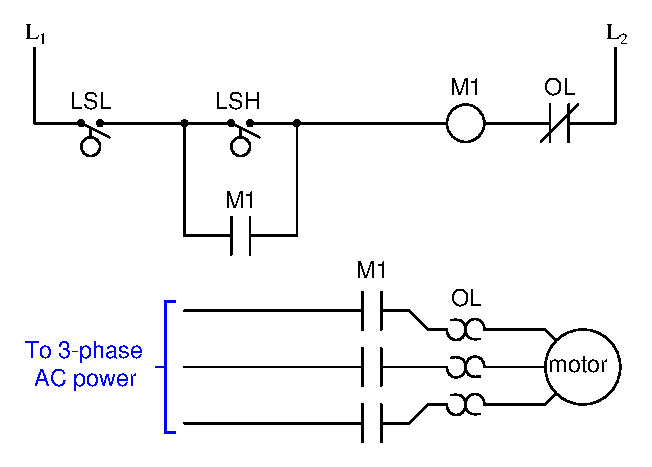
\includegraphics[width=15.5cm]{i00303x02.eps}$$

\vskip 20pt \vbox{\hrule \hbox{\strut \vrule{} {\bf Forslag til sokratisk diskusjon} \vrule} \hrule}

\begin{itemize}
\item{} Hva skjer hvis OL-bryteren feiler åpen i dette systemet?
\item{} Hva skjer hvis LSL-bryteren feiler åpen i dette systemet?
\item{} Hva skjer hvis LSH-bryteren feiler åpen i dette systemet?
\item{} Hva skjer hvis LSL-bryteren feiler kortsluttet i dette systemet?
\item{} Hva skjer hvis LSH-bryteren feiler kortsluttet i dette systemet?
\item{} Hva skjer hvis LSH-bryteren feiler kortsluttet i dette systemet?
\item{} Hva skjer hvis M1-holdekontakten feiler åpen i dette systemet?
\item{} Hva skjer hvis M1-holdekontakten feiler kortsluttet i dette systemet?
\end{itemize}

\underbar{file i00303}
%(END_QUESTION)





%(BEGIN_ANSWER)

Pass på å gjennomgå funksjonen til denne enkle motor start-stopp-kretsen i svaret.

%(END_ANSWER)





%(BEGIN_NOTES)

En kvikksølv-``tilt switch'' bruker flytende kvikksølv til å koble sammen ledningskontakter inni et forseglet glassrør når røret vippes i en bestemt retning.

\vskip 10pt

\noindent
Tankeeksperiment:

\begin{itemize}
\item{} Sump starter tom
\item{} Nivået begynner å stige
\item{} LSL-bryteren tipper; motor starter ikke ennå fordi LSH fortsatt er åpen
\item{} LSH-bryteren tipper; motor starter
\item{} Nivået begynner å falle når pumpen flytter avløpsvann ut av sumpen
\item{} LSH går tilbake til normal; motor fortsetter fordi styrekretsen er ``holdt inn''
\item{} LSL går tilbake til normal; motor stopper og forblir av til LSH tipper igjen
\end{itemize}

%INDEX% Lift station, wastewater treatment system
%INDEX% Process: wastewater lift station
%INDEX% Switch, level: tilting float (mercury)

%(END_NOTES)
